\documentclass[11pt]{article} % use larger type; default would be 10pt

\usepackage[utf8]{inputenc} % set input encoding (not needed with XeLaTeX)

\usepackage{tikz}
\begin{document}

% When this option is given, the node is not anchored on the last coordinate. 
% Rather, it is anchored on some point on the line from the previous coordinate 
% to the current point. The hfraction dictates how far on the line the point should be. 
% A hfractioni or 0 is the previous coordinate, 1 is the current one, everything else is in between. 
% In particular, 0.5 is the middle.

% The decision as to what constitutes the 'previous line' depends 
% on the previous path construction operation, in this case a line-to, or -- <coordinate> operation:

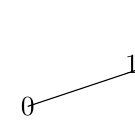
\begin{tikzpicture}
\path [use as bounding box, blue!30] (0,0) rectangle (1, 1);
\draw (0,0) -- (3,1)  % NOTE: this works ALSO when not drawing, .i.e. \tikz \path ..
	node[ pos=0] {0} 
	node[ pos=0.5 ] {1/2} 
	node[ pos=0.9 ] {9/10};
% \tikz \draw [use as bounding box, blue!30] (0,0) rectangle (1, 1);
\end{tikzpicture}


% The next case is the curve-to operation (the .. operation). In this case, 
% the "middle" of the curve, that is, the position 0.5 is not necessarily 
% the point at the exact half distance on the line. Rather, it is some
% point at \time" 0.5 of a point traveling from the start of the curve, where it is at time 0, 
% to the end of the curve, which it reaches at time 0.5. 
% The "speed" of the point depends on the length of the support
% vectors (the vectors that connect the start and end points to the control points)

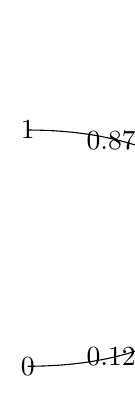
\begin{tikzpicture}
\path [use as bounding box, red] (0,0) rectangle (1, 4.3);
	\draw (0,0) .. controls +(right:3.5cm) and +(right:3.5cm) .. (0,3)
		\foreach \p in { 0 , 0.125 , ...,1}  
			{node[pos=\p]{\p}};
\end{tikzpicture}

% Another interesting case are the horizontal/vertical line-to operations |- and -|.
% For them, the position (or time) 0.5 is exactly the corner point.
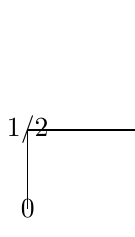
\begin{tikzpicture}
\path [use as bounding box, red] (0,0) rectangle (1, 2.3);
\draw (0,0) |- (3,1)
	node[ pos=0 ] {0} 
	node[ pos=0.5 ] {1/2} 
	node[ pos=0.9 ] {9/10};
\end{tikzpicture}

\begin{tikzpicture} 
\path [use as bounding box, blue!50] (0,0) rectangle (1, 1.6);
\draw (0,0) -| (3,1)
	node[ pos=0 ] {0} 
	node[ pos=0.5 ] {1/2} 
	node[ pos=0.9 ] {9/10};
\end{tikzpicture}
\end{document}